This chapter is a reprint of: \\
Zutshi, Apostolelli, Yang, Zheng, Dohi, Balzani, Williams, Savin, Buz\'{a}ki. \textit{Nature} \textbf{639}, 155--163 (2025). \\
DOI: 10.1038/s41586-024-08397-7

\section*{Abstract}

Neurons in the hippocampus are correlated with different variables, including space, time, sensory cues, rewards and actions, in which the extent of tuning depends on ongoing task demands. However, it remains uncertain whether such diverse tuning corresponds to distinct functions within the hippocampal network or whether a more generic computation can account for these observations. Here, to disentangle the contribution of externally driven cues versus internal computation, we developed a task in mice in which space, auditory tones, rewards and context were juxtaposed with changing relevance. High-density electrophysiological recordings revealed that neurons were tuned to each of these modalities. By comparing movement paths and action sequences, we observed that external variables had limited direct influence on hippocampal firing. Instead, spiking was influenced by online action plans and modulated by goal uncertainty. Our results suggest that internally generated cell assembly sequences are selected and updated by action plans towards deliberate goals. The apparent tuning of hippocampal neuronal spiking to different sensory modalities might emerge due to alignment to the afforded action progression within a task rather than representation of external cues.

\section{Introduction}

The hippocampus is often portrayed as a structure at the top of the relevant cortical hierarchy, which receives highly processed sensory modalities. It is assumed to synthesize those modalities into abstract space and time, explicitly reflected by the place and time fields of its neurons. Other considerations suggest that it is part of a top-down effector system involved in planning and initiating voluntary actions. In collaboration with frontal cortical areas, it can also sustain working memory, possibly related to the preparation for upcoming actions. Combining the sensory synthesis and effector systems supports effective navigation in an environment in the form of a predictive code. By disengaging from the environment, the hippocampus can support memory and planning.

Of these views, spatial navigation and sensory synthesis have received most attention. Yet, whether one framework can satisfactorily incorporate competing views and explain experimental data has remained a challenge. A critical problem is that the experimental design strongly influences the findings and their interpretation. By designing experiments in which space, time, action, memory or sensory modality is the relevant domain, one finds a description of place fields, time fields, reward cells, speed cells, tone cells, choice cells or `engram' cells in the hippocampus. The implicit assumption is that each label reflects unique computations performed by the hippocampus, generating `representations' specific to the relevant modality and reflecting different functions of hippocampal firing. Yet, a common confound is that the behaviour of animals becomes inevitably linked to the relevant domain. To disentangle task-specific sensory variables, motor actions and intentions, we designed a task that incorporated multiple behaviourally relevant domains and controls. By comparing similar movement trajectories and actions across task contingencies, we tested whether the firing of hippocampal neurons was driven by a general internal computation applied across all monitored modalities.

\section{Results}

\subsection{Mouse-controlled auditory navigation task}

We implemented an agent-controlled auditory navigation task to disambiguate tuning to spatial coordinates versus auditory tones. Mice (n = 6) ran on a linear track with 7 equally spaced water ports. During no-tone trials, they ran back and forth to collect water rewards at either end with no auditory tones playing. During tone trials, a tone ascended in frequency (2--25 kHz) in a closed-loop manner controlled by the spatial location of the mouse. The sweep gain between frequency and position was randomized from trial to trial so that the same frequency occurred at different spatial locations across trials. Mice must attend to the tone and lick at the closest water port whenever the target frequency (22 kHz) is reached. Return runs without a tone served as the control. Incorrect licks led to cessation of the tone and required the mouse to return to the home port to initiate a new trial. Thus, during tone trials, spatial (room) coordinates were uninformative because tones were the only predictor of reward location. Mice reached approximately 70\% performance within 3 weeks.

To confirm that mice attended to the auditory tones throughout the run, we implemented probe trials in two mice. Here the tones would abruptly truncate at either 4, 8 or 16 kHz, allowing us to estimate when the mice could successfully extrapolate the slope of the frequency change and predict the target port. Probe trials were randomly interspersed with tone trials at a likelihood of approximately 27\%. Although performance deteriorated at 4 kHz and 8 kHz, the 16-kHz probe trials were similar to controls, but there was variation in this performance across different ports. Thus, on average, mice could estimate and plan their approach to the target port between 8-kHz and 16-kHz tones.


\begin{figure}[htbp]
\centering
\includegraphics[width=\textwidth]{figures/ch_zutshi2025/fig1.png}
\caption[Agency-controlled auditory navigation task]{\textbf{Agency-controlled auditory navigation task.}
(a) Tone trials were preceded and followed by blocks of no-tone (NT) trials. During tone trials, the tone frequency was controlled by the spatial location of the mouse in a closed-loop manner.
(b) Trajectory of a mouse from an example session during tone trials; black circles denote trial start, red circles the trial end.
(c) Licks at various ports (black: no-tone licks; green: tone-correct licks; magenta: tone-incorrect licks; grey: other licks).
(d) Fraction of correct trials from six mice.
(e) Percentage of correct trials related to specific ports ($n=37$ sessions from 6 mice; Friedman test followed by Tukey--Kramer two-sided post-hoc tests, $\chi^2(5,175)=64.31$, $P=1.55\times10^{-12}$).
(f) Mouse-controlled tone frequency progression of each trial (grey lines) in time; average denoted in black; red dashed lines mark $-3$, $-2$, and $-1$\,s before the first lick.
(g) Random probe trials interspersed with tone trials; frequencies were cut off at 4, 8, or 16\,kHz.
(h) Performance during 4-kHz, 8-kHz, and 16-kHz probe trials (two-sided paired $t$-test, $n=6$ sessions from 2 mice; 4\,kHz: $t(5)=8.30$, $P=4.14\times10^{-4}$; 8\,kHz: $t(5)=3.08$, $P=0.028$; 16\,kHz: $t(5)=0.27$, $P=0.798$). $*P<0.05$, $**P<0.01$, $***P<0.001$.}
\label{fig:zutshi2025-fig1}
\end{figure}
\subsection{Non-spatial and spatial cell assemblies}

Mice were implanted with 128-site double-sided silicon probes in the CA1 pyramidal cell layer. We recorded a median of 235 neurons per session (83--372 cells; 8,113 cells total with $n = 6,220$ pyramidal cells and $n = 1,893$ putative interneurons out of 37 sessions in 6 mice). We first examined the activity dynamics of individual neurons as mice were solving the task. There were clear examples of cells whose discharge ramped up or down before the approach to any water port during tone trials. For descriptive purposes only, these neurons are referred to as tone cells based on a detected field in frequency space. In addition to this non-spatial frequency field, several cells displayed combinations of tone responses and a separate spatial place field. Although tone cell fields tiled the entire frequency landscape, there was a general overrepresentation of frequencies near the 22-kHz target. Tone cells constituted a significant fraction of all recorded CA1 cells (approximately 24\% of a median of 132 active pyramidal neurons per session; a total of 1,129 cells). Although many tone cells tended to have low-firing rates during no-tone trials, approximately 50\% of these cells also had stable place fields during no-tone trials. During error trials, we observed that the firing of tone cells was driven by the approach of the mouse to its chosen port rather than the assigned target for the trial, suggesting that such firing might reflect activity ramping up to the mouse-selected port (that is, the progression to the chosen port of the mouse) rather than auditory frequencies.

In addition to tone cells, there were clear examples of cells firing in fixed spatial coordinates regardless of the choice of the mouse and auditory tones. Upon closer inspection, these place cells were also modulated by the approach of the mouse to different ports during tone trials. During tone trials, several cells shifted or expanded their place fields with varying run lengths. These results suggest that rather than belonging to unique functional cell classes, both tone cell and place cell neurons can have mixed spatial and non-spatial properties.

To quantify to what extent cells were co-modulated by space and progression to the chosen port, we used a Poisson generalized additive model (P-GAM), which modelled the average response of a neuron as a function of continuous behaviour variables such as spatial position during no-tone and tone trials and the progression to the choice port (or tone frequency). Almost 60\% of the cells were co-tuned to both position and tone frequency. The ratio of the mutual information for position versus frequency revealed a continuous distribution, establishing that rather than existing as discrete functional classes, most cells exhibited tuning preferences lying along a continuum. Consistent with this idea, place cells and tone cells displayed prototypical properties of hippocampal cells, such as theta-phase precession and theta compression, with place and tone cells co-firing within the same theta cycle.

Given the mixed nature of neuronal responses, we identified assemblies of co-firing neurons using independent component analysis that were not limited to functionally defined classes. Approaches to distinct ports were associated with similar assembly sequences, but the target warped their temporal dynamics. Linking these assemblies back to functional types, we observed that assemblies active early in a trial contained mostly place cells, whereas those at the end mainly contained tone cells. In addition to modulation of hippocampal firing between different tone trials, we also observed significant remapping from no-tone (NT1) to tone trials, but not during return runs, indicating context-dependent hippocampal patterns. To address the source of remapping, we trained a separate cohort of mice on a control task in which the reward was kept fixed to the end port even during tone trials. Therefore, auditory sweeps were identical but had no task-related significance. As expected, there was a time-proportional drift in neuronal firing throughout the session, yet no remapping was observed between NT1 and tone trials. Thus, sound alone could not explain the remapping.

Mice ran stereotyped trajectories during no-tone trials, mainly along the wall of the track without water ports. By contrast, during tone trials and the second block of no-tone trials, the running trajectories were consistently closer to the wall with middle ports, reflective of the search by the mouse for the correct ports. We regarded the linear track as two-dimensional space and examined the impact of minor deviations. A similar decorrelation was observed between NT1 and tone trials in the two-dimensional maps. We hypothesized that the sequence of positions (where the mice are coming from or are planning to go) was responsible for the decorrelation. We used hierarchical clustering to classify the movement trajectories in the forward running direction into two groups: away from the middle water ports or closer to the middle water ports. Rate maps, averaging trials for each movement trajectory group and condition (tone versus no tone), were separately generated and correlated. Different movement trajectories yielded significantly different firing patterns within the same task conditions. However, even the same trajectories but in different conditions led to remapping, pointing to the impact of task engagement to remapping.


\begin{figure}[htbp]
\centering

\includegraphics[width=\textwidth]{figures/ch_zutshi2025/fig2.png}
\caption[Conjunctive non-spatial and spatial neuronal responses]{\textbf{Conjunctive non-spatial and spatial neuronal responses.}
(a) Three example CA1 pyramidal cells displaying tone (left), mixed (middle), and place (right) tuning. Trajectories by trial type (top) and average firing rate heatmaps for position and frequency (bottom).
(b) Tone cells ordered by frequency preference, showing faint port modulation during no-tone trials.
(c) Relative weights of neurons for two example assemblies detected using ICA; grey refers to other cells.
(d) Activation profile of all assemblies from an example session against the first detected lick during tone trials (top), with PSTHs for assemblies 1 (green) and 2 (blue) shown (bottom).
(e) Sum of weights of place cells (black) and tone cells (pink) averaged by the time bin of peak activation of each assembly against the first lick. Assemblies active early in a trial were place cell dominated; those preceding the lick were tone cell dominated ($n=33$ sessions from 6 mice; Wilcoxon two-sided signed-rank test). $*P<0.05$, $***P<0.001$.}
\label{fig:zutshi2025-fig2}
\end{figure}
\subsection{Effect of external variables on firing}

Examination of error trials revealed that firing was not driven by auditory tones but rather by the choice of the mouse. Nonetheless, it is possible that tone cell firing reflected the `belief' of the mouse or falsely perceived tones. We thus examined the activity of tone cells during probe trials, in which the tone ramp was terminated at 4 kHz. Despite the truncated auditory cue, tone cells continued to ramp after the termination of the tone while the mouse approached the port. The spatial map, cell assemblies and neural sequences also remained stable despite the truncation of auditory cues. Thus, neuronal firing was not induced and sustained by sound per se. Instead, the findings can be more parsimoniously explained by an internally generated sequence towards an upcoming choice.

We observed no reliable relationship between firing rates and speed, suggesting that tone cells were not modulated by speed. Because most tone cells fired immediately before approaching a water port, we next considered whether they were directly responding to the presence of the reward. However, we found no difference between correct (water reward delivered) and incorrect (no water reward delivered) trials up to the first detected lick. To further explore the extent to which rewards, or their expectation, might affect firing, we compared firing patterns on return runs. Throughout training, mice were rewarded at the home port only if the trial was correct and unrewarded after incorrect choices. Despite the expectation of the reward presumably being different between correct and incorrect trials, we observed no differences in cell firing on the return runs. To follow up on these results, we designed a new task. Mice were trained to run back and forth on a linear track with a reward port only at one end (666 cells total with $n = 527$ pyramidal cells and $n = 139$ putative interneurons in 2 sessions of 2 mice), therefore never having received a reward at the other end. Midway through the session, rewards were provided at both ends of the track. No changes in hippocampal firing were observed upon the introduction of the reward, suggesting a limited direct influence of rewards on hippocampal firing.

Finally, we asked whether the expectation of reward altered firing patterns by separating the type of licks the mouse performed. We grouped licks into five classes: (1) `choice licks', the first detected lick on a tone trial, which included both error and correct licks; (2) `no-tone licks', the licks at port 6 during no-tone trials; (3) `spontaneous forward licks', mice sometimes sampled other ports during the no-tone trials or after choosing in tone trials; these spontaneous licks had no associated tasks, tones or rewards and may have reflected exploration or validation; (4) `spontaneous reverse licks', same as type (3) but occurred as the mouse returned to the home port, meant to control for running direction and stereotyped motor movements; and (5) `home port licks', the first lick detected at the home port that initiated the subsequent trial. Spontaneous (exploration) licks were preceded by ramp firing similar to choice licks. Only weak responses were observed for no-tone licks, and the smallest response was for homeport licks, suggesting that firing was not a uniform reward-expectation signal but distinct between habitual and task-modulated licks. During tone trials, neuronal responses were not uniformly distributed across the approaches to all ports. Because the number of possible options sequentially decreased with every port crossed, the probability of a correct choice increased for later ports. Spiking preceding licking at earlier (low-probability) ports was stronger, and progressively diminished for later (high-probability) ports. Neuronal firing, therefore, reflected a prediction signal for evolving action outcomes, modulated by expectation, similar to the postulated role of dopamine.


\begin{figure}[htbp]
\centering

\includegraphics[width=\textwidth]{figures/ch_zutshi2025/fig3.png}
\caption[Non-spatial firing is not driven by tones or rewards]{\textbf{Non-spatial firing is not driven by tones or rewards.}
(a) Example CA1 pyramidal tone cells during non-probe and probe trials (truncated at 4\,kHz). Progression to choice refers to normalized distance to the choice port.
(b) Tone cells sorted by tuning location during non-probe trials.
(c) Cell-by-cell correlations for the cells in panel b versus shuffled data. Activity remained stable despite tone termination ($n=362$ cells, 8 sessions in 2 mice; Wilcoxon two-sided rank-sum test, $z=23.23$, $P=2.09\times10^{-119}$).
(d) Lack of reward effect: only one end was rewarded for 40--60 trials, then a second reward was introduced.
(e--f) Place cells sorted on the one-port condition and maintained between conditions for forward (e) and return (f) runs.
(g) Cell-by-cell correlation of rate maps for 10-trial blocks; reward introduced after block 5.
(h--k) PSTH of a tone cell by port approach (h); spiking during no-tone trials with spontaneous licks (i); spiking during correct and incorrect tone trials (j); average PSTH separated by lick types (k).
(l) Average rate within $\pm 0.3$\,s around the first lick ($n=565$--633 cells from 6 mice; Kruskal--Wallis test followed by Tukey--Kramer two-sided post-hoc tests, $\chi^2(4,3079)=330.90$, $P=2.33\times10^{-70}$).
(m) Fraction of cells per session firing significantly before approach to ports 1--6 during tone choice licks ($n=37$ sessions from 6 mice; Friedman test, $\chi^2(5,180)=35.44$, $P=1.23\times10^{-6}$). $*P<0.05$, $**P<0.01$, $***P<0.001$.}
\label{fig:zutshi2025-fig3}
\end{figure}
\subsection{Population activity and behavioural goals}

To understand how the combined firing of neurons could be related to behavioural decisions, we examined hippocampal firing across the population. The activity of all recorded cells was binned into 100-ms time bins and visualized by the dimensionality reduction technique uniform manifold approximation and projection (UMAP). Each population vector time bin on this lower-dimension manifold was colour-coded according to behavioural variables, such as the spatial position or the direction of running. The manifold mirrored the geometry of the spatial environment, with unique segregations between forward and reverse runs. By selecting the correct forward runs during tone trials and colouring by spatial position, auditory tones or target ports, we observed that the neural trajectories diverged from the main branch before the mice approached the target port. We observed similar results across mice and sessions with varying numbers of simultaneously recorded neurons.

To examine how neural firing relates to the branches on the neural manifold, we sorted neurons using an unsupervised clustering analysis and found reliable cell assembly sequences across trial types. To quantify how these assemblies related to the manifold shape, we implemented a two-dimensional Bayesian decoder to simultaneously predict the position of the mouse and the chosen port (`goal') in 10-ms time bins. Each analysis method, including the UMAP display, cell sequences and Bayesian decoding, showed a similar evolution of neural activity for port-specific runs, including error probe trials. Specifically, the chosen port by the mouse could be predicted for 85\% of trials, approximately 1.1 s before the lick. To relate this decoding time point to branches on the neural manifold, we used a change-point detection algorithm to identify consistent epochs of decoding prediction. The time point of the last-detected epoch generally occupied the branch points of the manifold for each port. The average tone frequency at this time point was between 8 kHz and 12 kHz, corresponding to the frequencies when the mice predicted the target port on probe trials. Decoding preceded changes in running speed. Thus, the goal-specific modulation of place and tone cells led to a population-level code that corresponded to the upcoming actions of the mouse.


\begin{figure}[htbp]
\centering
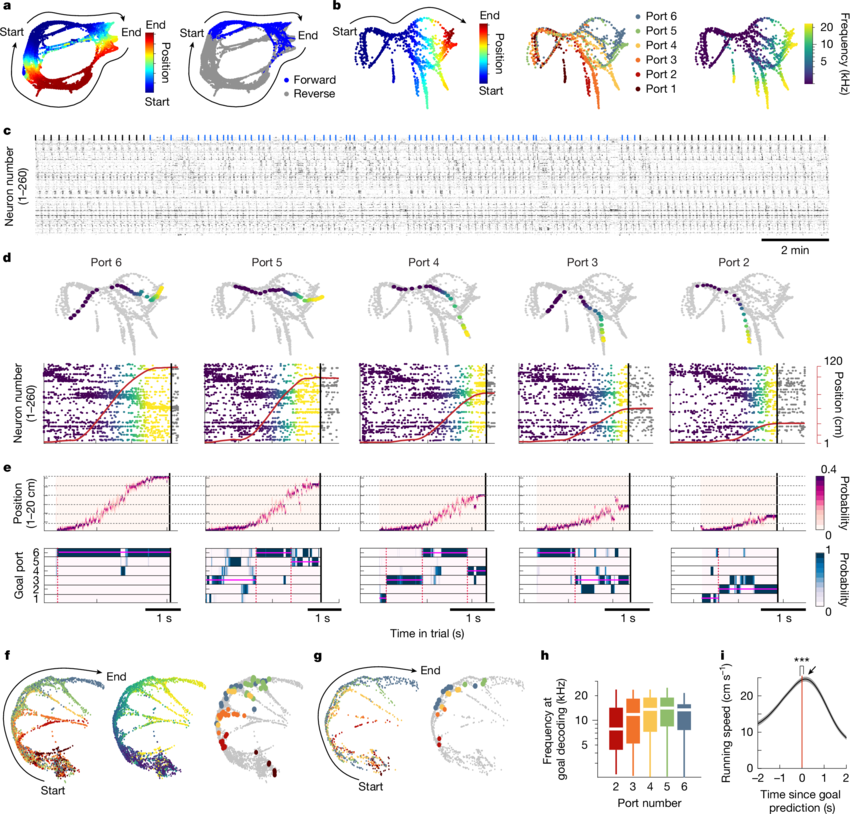
\includegraphics[width=\textwidth]{figures/ch_zutshi2025/fig4.png}
\caption[Hippocampal CA1 activity predicts upcoming choices]{\textbf{Hippocampal CA1 activity predicts upcoming choices.}
(a) Neural activity from an example session ($n=372$ cells) binned into 100-ms time bins and visualized on a UMAP manifold, coloured by position (left) and running direction (right).
(b) Manifold from correct forward tone trials, coloured by position (left), target port (middle), and auditory frequency (right).
(c) Spike raster of pyramidal cells sorted by rastermap; ticks denote start of no-tone (black) and tone (blue) trials.
(d) UMAP overlaid with single trials coloured by auditory frequency, with corresponding spike rasters.
(e) Position decoding (top) and goal decoding (bottom) within individual trials; black vertical line: first lick; red vertical dashed lines: significant change points; pink horizontal line: mode goal decoded between two change points.
(f--g) UMAP coloured by target port, tone frequency, and timestamp of final change point for a different mouse on correct trials (f) and 4-kHz probe trials (g).
(h) Average tone frequency at which the decoder settled onto its final change point by port ($n=158$--346 decoded trials).
(i) Goal decoding preceded running speed peak ($n=37$ sessions from 6 mice; Wilcoxon two-sided signed-rank test, $P=2.69\times10^{-4}$). $***P<0.001$.}
\label{fig:zutshi2025-fig4}
\end{figure}
\subsection{Within-trial evolution of action plan}

We reasoned that if hippocampal activity reflected action plans, we could trace how such action plans are shaped within a trial. We identified moments of peak deceleration in the speed profile of the mouse when it approached the chosen port or crossed previous ports. These transient deceleration events were often accompanied by brief head turns towards the port under consideration (termed `deliberation'). During deliberative but not during other decelerations on the track, tone cells briefly ramped their activity but quickly stopped spiking, corresponding to the mouse passing the port, which was also accompanied by a sudden jump in goal decoding and flickering of tone cell assemblies. Although choice decelerations deeply extended into the manifold branches, deliberation neural trajectories only briefly entered the relevant manifold branch and exited back out. In addition, the likelihood of the position of the mouse being decoded beyond the next port was significantly higher if the mouse was going to pass an upcoming port---an effect that was not dependent on the speed of the mouse but on its position `lookahead' during the ascending phase of the theta cycle. Thus, goal-specific signals were modified dynamically with ongoing action plans.


\begin{figure}[htbp]
\centering
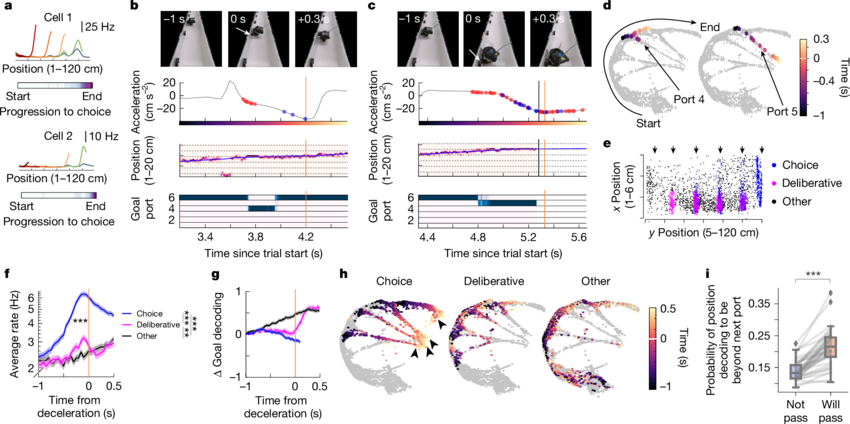
\includegraphics[width=\textwidth]{figures/ch_zutshi2025/fig5.png}
\caption[Action plan decoding in single trials]{\textbf{Action plan decoding in single trials.}
(a) Two example tone cells: spatial firing (top) and average progression-to-choice map (bottom).
(b--c) Example events from a single trial showing behavioural ``checking'' of port 4 (b; no lick) and licking at correct port 5 (c). Rows show: video frames, acceleration profile (yellow: acceleration minimum; red/blue dots: spikes from cells 1 and 2), position decoding, and goal decoding.
(d) UMAP display for the single trial shown in panels b and c; coloured dots denote time windows.
(e) Significant decelerations during forward runs, clustered into choice (blue), deliberative (pink), and other (black) categories. Only ports 3--6 considered to allow for deliberation at previous ports.
(f) Average tone cell firing around detected deceleration moments ($n=633$ cells; Friedman test followed by Tukey--Kramer post-hoc tests, $\chi^2(2,1264)=399.23$, $P=2.04\times10^{-87}$).
(g) Change in goal decoding compared with predicted goal at $-1$\,s; sudden shift for deliberative decelerations.
(h) Significant decelerations separated by category on the UMAP; arrowheads denote chosen ports 3--6.
(i) Probability of position decoder predicting beyond the upcoming port was significantly higher if the mouse would pass versus lick at the port (Wilcoxon two-sided signed-rank test, $P=2.91\times10^{-11}$; $n=37$ sessions, 6 mice). $***P<0.001$.}
\label{fig:zutshi2025-fig5}
\end{figure}
\section{Discussion}

We studied how hippocampal neurons vary their apparent tuning to various modalities in a paradigm where space, auditory tones, rewards and contexts were juxtaposed. We observed correlations between firing patterns versus spatial position, time, auditory modalities, reward and context. Yet, in agreement with experiments that attempted to identify modality-specific or abstract space responses, we found that the dominance of particular correlations depends on task demands and, therefore, varies across experiments. Analysis of the movement paths of the mice uncovered that hippocampal firing was linked to prospective action patterns and modulated by goal expectation rather than tuning to the relevant sensory modalities. We hypothesize that the previously reported apparent hippocampal tuning to abstract cognitive variables can be grounded in a framework in which neuronal firing reflects an internally generated action plan afforded by the environmental conditions of the mouse.

Although adjusting the target frequency of the discriminative sound by the mouse was a critical task variable, our analysis revealed that it was not the `sound landscape' that brought about the firing changes of hippocampal neurons but, instead, the specific actions taken by the mouse. First, tone-responding neurons increased their discharge at sampled water-port locations during no-tone trials. Second, during error trials, the firing pattern of the neurons reflected the progression of the mouse towards the erroneously chosen port rather than the auditory frequencies. Third, when the tone ramp was terminated at 4--16 kHz on probe trials, neuronal firing continued to ramp similarly as the mouse approached the port. Finally, the firing patterns of hippocampal neurons `remapped' across tone and no-tone trials of the main task. Yet, the presence of the same auditory sweep with no consequence on securing the reward had no effect on neuronal firing in control experiments. We hypothesize that the role of the discriminative `go' signal is to select an action sequence with an associated neuronal trajectory, which proceeds according to internally organized motives, possibly modified during learning, rather than continuously controlled by sensory cues. How learning shapes such internal dynamics remains an interesting question for future studies.

An alternative explanation of our findings is that neuronal trajectories were influenced and scaled by the presence of the reward and its expectation. Consistent with this idea, hippocampal neurons started to ramp up their firing rates before licks, independent of the location of the mouse on the track or the presence of a tone. Yet, control experiments distinguished firing pattern correlates of reward and sensory cues from motor responses at both the single-neuron and the population levels. First, the ramping of lick-responding neurons was identical during rewarded and either erroneous or learned non-rewarded trials, demonstrating that reward expectation and consumption were not critical. Second, in the tone task, neurons that robustly responded before licking also responded before exploratory licks but only weakly in the no-tone task despite involving the same motor patterns. Conversely, very few tone cells responded before home port licks, even though they resulted in the same volume of water as rewarded tone or no-tone trials. In addition, the fraction of responding neurons and the magnitude of the responses were different between ports. Finally, tone cells fired even during hesitation or deliberation without licks. Thus, neither the reward per se nor the simple motor information could explain hippocampal neuronal firing patterns, which are better explained by deliberative and intentional actions towards goals.

Several observations support the action plan hypothesis. Sequences of cell assemblies consistently evolved approximately 1 s before the choice, including probe trials. Early in the trial, assemblies were dominated by place cells and gradually replaced by tone cells. Although these labels approximate the experimenter-established relationships, they do not imply distinct mechanisms. We observed reliable goal decoding and branches on the manifold emerging at a similar timescale, coinciding with the approximate frequency at which mice made decisions. Together, our findings align better with an interpretation that the discriminative signal selected a neuronal sequence (or trajectory), which proceeded according to internally organized motives that guided the current action plan of the mouse. This view is supported by the observation that the hippocampus continues to generate the same fractions of place cell sequences even in the absence of the grid cell-supporting medial entorhinal input. Building on previous research, we hypothesize that external cues do not continuously drive neuronal spikes in the hippocampus but rather serve to select and update pre-existing (or attractor) trajectories appropriate to a given task phase.

The hypothesis of neuronal sequence-sustained internal goals is supported by previous observations demonstrating that the extent and forms of neuronal sequences in the hippocampus correlate with the direction and distances of the animal-set goals. Our findings are also relevant to rescaling place cells with changes in the size of the environment and the intrinsic switching of their fields between reference frames, as well as to goal-predicting `splitter' cells and prediction in general. Each of these independently studied features may reflect the same underlying physiological mechanism if hippocampal firing is viewed from the lens of a dynamical sequence generator that progresses towards a task-related goal. Although our results primarily pertain to non-spatial aspects of firing, we hypothesize that similar action sequences may also underlie spatial firing that is sensitive to precise trajectories and the goals of the animal.

In our experiments, the evolving internal goals were reflected by the quantal jumps of the population activity from port to port and associated behavioural deliberations (brief head movements) of the mouse.

The concept of a goal expands beyond a mere physical location and encompasses any inherent end point that leads to a desired outcome, as implied by experiments in humans. Despite the vagueness of these terms, the distinction between reward and goal is subtle yet crucial, shifting the focus from an external stimulus or location to an internally driven, intentional and deliberative target. Departing from the notion of `representation' of external stimuli or `mapping' the environment onto the hippocampus, we hypothesize that its internally generated dynamics are projected onto the niche of the animal to make sense of the world through its prospective actions.

\section{Methods}

\subsection{Experimental animals}

The Institutional Animal Care and Use Committee at New York University Langone Medical Center approved all experiments. Mice were housed in fully equipped facilities in the New York University School of Medicine Science Building. Mice were housed at around 22 °C, with a relative humidity of approximately 45\%. The mice were on a 12-h light--dark cycle and were housed 4--5 per cage before implantation. Upon the onset of behavioural training and subsequent surgery, the mice were moved to a 12-h reverse light cycle (lights on or off at 19:00 or 07:00, respectively) and housed individually. Mice were provided food and water ad libitum but were water restricted to maintain 80\% of their weight during and after behavioural training. We used a combination of transgenic and wild-type male mice (auditory task; $n = 6$ male mice, of which 4 were double transgenic mice crossed between Pvalb-IRES-Cre females (Jax Stock no. 017320) and Ai32 males (Jax Stock no. 024109); the other two mice were C57BL/6J wild types (Jax Stock no. 000664); and for the control task, $n = 3$ male mice of which 1 was double transgenic as described above, and 2 were wild type). No obvious differences in behaviour or neural firing emerged between the two types of mice. At the time of implantation, mice ranged from 3 to 6 months of age and 22--31 g in weight. For the variable reward task, $n = 2$ male mice of which both were double transgenic as described above.

\subsection{Surgical procedures}

Mice were implanted with 128-channel silicon probes (ASSY-INT128, Diagnostic Biochips) into CA1 (for task mice, one mouse was implanted with a P128-6 probe, whereas five mice were implanted with P64-1-D Janus double-sided probes; for control mice, one mouse was implanted with a P128-6 probe, whereas two mice were implanted with P64-1-D Janus double-sided probes). For all surgical procedures, mice were induced with 2.5--3\% isoflurane in oxygen anaesthesia (SomnoSuite Low-Flow Anesthesia System) and placed in a stereotaxic apparatus (Kopf Instruments). The level of isoflurane was then decreased to 1.3--1.5\% for the remaining surgical procedures. During the surgery, body temperature was maintained at 37 °C using a heating pad (Physitemp, TCAT-2LV Animal temperature controller). Vaseline was applied as eye lubricant. Following no reaction to toe pinch, a small incision was made in the scalp, the scalp was cleaned with iodine (Dynarex Povidine Iodine solution) and lidocaine cream (Ferndale LMX4) was locally applied. The skull was then scored using a scalpel to ensure adhesion to the headcap. The coordinates used for CA1 were --1.9 mm anteroposterior and +1.6 mm mediolateral from bregma. A ground screw coupled with a 0.005″ stainless steel wire (792800, A-M Systems) was implanted in the skull above the cerebellum. Next, a base plate was cemented to the scored skull surface using Metabond (S380, Parkell C\&B). The probes were mounted on custom-made metal microdrives to allow precise adjustment of vertical position of sites after implantation. During surgery, probes were implanted at the level of the cortex (0.4 mm dorsoventral). A combination of mineral oil (O121-1, Fisher Chemical) and paraffin wax (18634, Sigma-Aldrich; melted in a 1:1 ratio) was used to seal the craniotomy and cover the probe shanks. In the transgenic mice, four 200-µm optic fibres were also implanted in the brain, but sessions when those stimulations were performed were not included in this paper. The microdrive was cemented on the metabond skull surface using a combination of light-cured and regular dental cement (Unifast LC, Unifast Trad). Finally, a custom 3D-printed grounded copper mesh hat was constructed, shielding the probes. Following surgery, an NSAID analgesic was injected (Ketoprofen at 5 mg kg$^{-1}$, approximately 0.13 ml for a 25 g mouse, stock solution of 1 mg ml$^{-1}$, subcutaneous). Mice were allowed to recover and were continuously monitored for at least 1 week before water restriction and behavioural training resumed. Body weight was monitored for all the days following surgery. The position of the probe was confirmed at the end of each experiment. The mice were perfused with cold saline solution (0.9\%) followed by pre-made 4\% paraformaldehyde in PBS solution (Affymetrix USB). Brains were post-fixed for 24 h in 4\% paraformaldehyde and sectioned coronally to visualize the hippocampus. Sections were obtained with 40--50 µm thickness using a vibrating blade microtome (VT1000S, Leica), mounted on electrostatic slides, coverslipped with DAPI Fluoromount-G (0100-20, Southern Biotech), and imaged using a virtual slide microscope (VS120, Olympus). No additional immunohistochemistry or tissue processing was done to visualize the probe tracks.

\subsection{Behavioural apparatus and task description}

We constructed a linear track using white acrylic (1/8″ thick) with dimensions of 120 cm (length) × 7.5 cm (width), with 5-cm high walls. The track contained seven equally spaced (20 cm apart) water ports. The home port and port 6 were located on the short walls of the track, whereas ports 1--5 were located along one of the long walls of the track. Water was delivered through blunt 18-G needles connected (using Tygon E-3603 Tubing; 1/16″ ID, 1/8″ OD) to solenoid valves (EW-98302-02, Cole-Parmer) that were briefly opened for 30 ms. The needle was positioned precisely within a U-shaped infrared (IR) sensor (HiLetgo LM393 Correlation Photoelectric Sensor), such that any licks on the needle would break the IR beam. Successive breaks at the same port during a visit were disregarded during analysis. A speaker (MakerHawk Mini Speaker, 3 W 8Ω) was positioned above port 6, facing the home port, and was calibrated to ensure that it played frequencies up to 25 kHz (60--80 dB SPL; 20 dB roll-off between 2 kHz and 25 kHz).

Water delivery and the tones were controlled by a combination of Bonsai (https://bonsai-rx.org/) and a custom-made Arduino circuit. A Basler overhead camera (acA640-90gc, Graftek Imaging) acquired images with a frame rate of 30 Hz. Bonsai was used to detect the real-time position of the mouse by contrasting the black fur of the mouse against the white maze. This centroid position was sent to Arduino using the serialStringWrite function. The Arduino would randomly assign a target port for a trial and rescale the Bonsai-detected position of the mouse to the distance between the home and the target port. For example, if the target port was 6 (located 120 cm from the start location), and the current position of the mouse was at 60 cm, the instantaneous normalized position was 60/120, that is, 0.5. However, if the target port was 4 (located 80 cm from the start location), the normalized position became 60/80, that is, 0.75. Auditory frequencies were linked to this normalized position according to the following formula:

\[
F = f_0 \cdot \left(\frac{f_{target}}{f_0}\right)^x
\]

where $F$ = current frequency, $f_0$ = 2 kHz, $f_{target}$ = 22 kHz and $x$ is the current normalized position. The frequency sweep was designed to increase logarithmically from 2 kHz, with the target port coinciding with a frequency of 22 kHz. Although tones could continue beyond the target, because of the limitations of the speaker, frequencies beyond 25 kHz were not accurately delivered if the mouse overshot, but these were rare instances. Tones were delivered using the Arduino Tone() function, which generated square pulses modulated at the specified frequency. Microphone (AU-PM422, MAONO; sampling rate up to 192 kHz) recordings ensured that auditory frequencies were playing as designed and the resultant sound spectrogram was inspected using Audacity.

\textit{Acoustic cue-guided navigation paradigm.} During no-tone trials, mice ran along the linear track, receiving water at the two ends of the track, that is, port 6 and the home port. In the tone trials, licking at the home port initiated a tone of 2 kHz that ascended logarithmically in a closed loop with the position of the mouse. A correct lick response triggered the solenoid, and the tone stopped playing. We ensured that the delay between the mouse touching the spout and the transistor--transistor logic (TTL) pulse of the lick was not greater than 33 ms (corresponding to 1 frame-rate cycle of the Arduino) and corrected this delay in our analysis. After a choice, mice were free to sample other ports (unrewarded checks) before returning to the home port to lick to initiate the next trial. If the previous trial was correct, mice also received a water reward at the home port. However, if the previous trial was incorrect, both the choice lick and the subsequent home port lick were unrewarded. An incorrect lick response in the tone trials was followed by a 1-s long 3-kHz error tone.

\textit{Probe trials.} In two mice, probe trials were randomly interspersed with regular (non-probe) trials at approximately 30\% probability, but only if the target was port 3, 4, 5 or 6. This criterion was introduced because ports 1 and 2 did not allow enough separation in terms of distance between the truncation of tones and the target port. Within a session, a cut-off frequency was pre-determined as 4 kHz, 8 kHz or 16 kHz, after which tones stopped playing with a trial. A correct probe trial was if the mouse correctly extrapolated the sweep speed and licked at the target based on the short, truncated sweep. Other licks were classified as incorrect. For electrophysiological recordings, only 4-kHz probe trials were used to maximize the duration when sounds were off.

\textit{Control task paradigm.} To control for auditory cues, three mice were trained to run back and forth on the same track with the same task structure as previously described. However, only the two ports at either end were rewarded. Tones would stop playing after 25 kHz. Return runs did not have any tones associated with them. For comparison with the mice performing the task, recordings were only analysed after mice had been performing the control version of the task for at least 7 days. This ensured that there were no effects due to the novelty of the auditory cue and that mice had learned that the tones were irrelevant.

\textit{Variable reward paradigm.} Mice had previously been trained to run in the auditory navigation task. After collecting data on that task, mice were kept in their home cage for 3--4 weeks. They were then introduced to a novel linear track of similar dimensions (110 cm long, 6 cm wide). Recordings were analysed on the first day of this task. For the first approximately 60 trials, only one end was rewarded. Midway through the task, and without interruptions, a second reward was introduced at the opposite end of the track.

\subsection{Behavioural training and analysis}

On days when behavioural sessions were performed, the mice were deprived of water and only received water during the sessions. On other days, the mice were provided 2 ml of water. Body weight was monitored on all days, and the water schedule was interrupted if the body weight reached below 80\% of the starting weight. Before implantation, mice were pre-trained to perform the task until they reached 65\% accuracy. The stages of training included: (1) habituation to the track and water ports, so that mice learned to poke to trigger water rewards (approximately 2 days). (2) Linear track training in which mice received a water reward at either end after poking and reached up to 60--70 trials (approximately 3--4 days). (3) Autoshaping, in which tones would increase in a closed loop to the position of the mouse, but the water reward would automatically be released at the target port without the mice having to nose poke. Incorrect licks were also not penalized (approximately 2 days). (4) Training to abstain from licking at incorrect ports. Only one port was assigned the target in this stage, generally port 3. Mice must poke at the target to receive water rewards, and licks at earlier ports would result in incorrect trials. This would often be the most variable stage between mice. If mice did not adapt their behaviour after 100 trials, the first few ports would be physically blocked to train the mice to abstain from premature licks (approximately 3--4 days). (5) Expanding phase 4 to a few more ports, usually ports 1--3, or ports 3 and 6 (3--4 days). (6) The final version of the task with all ports rewarded (approximately 3--4 days). Mice transitioned between stages 4 and 6 if they reached 65\% at each stage. The entire training from start to finish would usually take approximately 3 weeks. Following surgery, mice were retrained starting from stage 4 but would quickly transition to stage 6 within 3--4 days.

To quantify the performance of the mice, the proportion correct and proportion incorrect was calculated for each target port separately. The performance was calculated as the fraction of correct licks at a given port relative to the total number of trials where that was the target port. The proportion of incorrect trials was calculated as the fraction of trials when a given port was incorrectly chosen relative to all trials where that port was not the target.

\subsection{Electrophysiological recordings, unit clustering and neuron classification}

Electrophysiological data were acquired using an Intan RHD2000 system (Intan Technologies) digitized at 30 kHz. The wideband signal was downsampled to 1,250 Hz and used as the local field potential. A pulley system was designed to counteract the weight of the tether and headstage. The position of the mouse was recorded using an overhead Basler camera (acA1300-60 gmNIR, Graftek Imaging) sampling at 30 Hz. A front camera recorded the forward running direction of the mouse for additional behavioural analysis. Camera videos were synchronized with neural data with TTLs signalling shutter position. Digital inputs to the Intan RHD system provided timestamps for TTLs from lick ports and water delivery from the solenoids.

Spikes were extracted and classified using Kilosort using a custom pipeline KilosortWrapper. Automated sorting was followed by manual curation of the waveform clusters using Phy and custom plugins for Phy. Kilosort clustering was performed with specified parameters. Units were separated into putative pyramidal cells and narrow waveform interneurons using their autocorrelograms, waveform characteristics and firing rate. This classification was performed using CellExplorer.

\subsection{Rate map generation}

1D spatial rate maps were generated by binning spiking data into 2.5-cm wide bins, generating maps of spike counts and occupancy for periods when the speed of the mouse was more than 0.1 cm s$^{-1}$. A rate map was constructed by dividing the spike map by the occupancy map and smoothing it with a 5-bin Gaussian filter. For tone trials, forward direction maps used time windows between the start of the trial (home port lick) and the end of the trial (first detected lick on the trial). Maps for the reverse direction runs included time windows between the end of a trial (first detected lick) and the subsequent home port lick. Because the mouse behaviour was more variable during the return runs, an additional speed criterion was applied (speed < --2 cm s$^{-1}$) to ensure movement in the reverse direction.

1D frequency or choice maps were constructed by rescaling the spatial position of the mouse to match the trajectory length within a trial. The relevant port was generally considered to be the port where the mouse first licked but was the assigned target port for the error trial analysis. For frequency maps, frequency was estimated using equation (1). Rate maps were generated as described above but by binning spikes along the choice variable. For tone trials, average maps for ports 1--6 were first constructed separately, and then these average maps were averaged further to generate overall tuning across tone trials.

2D spatial maps were generated by making 1-cm wide bins and binning across both the $x$ and the $y$ spatial positions. Smoothing involved a 5 × 5 bin Gaussian filter.

\subsection{Field detection}

\textit{Place cells.} Place fields were defined from the above-described rate maps using a combination of peak detection and across-trial correlation methods. Only pyramidal cells were used. The field boundaries were defined for cells with a minimum peak firing rate of 5 Hz, and extended until the rate was above 20\% of the peak firing rate. The width of the field was required to be between 8\% and 70\% of the size of the rate map. All cells that had a detected field using these criteria in spatial rate maps were included as place cells. For the place field modulation by run length analysis, cells were only included if they had a place field in the rate map generated by averaging across port 2--6 tone trials as well as a field within 30 cm of this averaged field for each individual trial type.

For the correlation metrics across no-tone and port 6 tone conditions, as well as the trajectory analysis, cells were included if they had a field in either no-tone or port 6 tone maps. Spatial rate map correlations for individual cells between conditions were calculated as the average pixel-by-pixel Pearson correlation coefficient of the smoothed-averaged firing rate maps. Rate map stability was defined by generating rate maps for the first and second halves of each condition and correlating these half-session rate maps.

\textit{Tone cells.} For tone cells, cells were selected with the same criteria as place cells to have a field in the averaged frequency maps. To ensure that these cells were firing robustly across trials, the frequency maps across ports 1--6 were correlated to each other and additionally required a correlation value > 0.1. For reward responses, peri-event time histograms around lick events were generated separately for each port for tone cells by binning spike rates in 100-ms bins. To focus on cells firing around the reward location, only cells with a field within the last 10 bins were used for the analysis. Speed analysis was performed by calculating the instantaneous firing rate of tone cells within 100-ms bins and calculating the Pearson's correlation coefficient of the rate with running speed.

\subsection{Movement trajectory clustering}

The movement trajectory of the mice along the width of the track was clustered by using agglomerative hierarchical clustering. The $x$ position along the width of the track within a trial was downsampled to 7 points (each point corresponding to the $y$ position of a water port) for all no-tone and port 6 tone trials. This array representing individual $x$ position trajectories was clustered into paths according to their Euclidean distance. Only a maximum of two clusters was allowed. Two sets of average rate maps were therefore generated for each condition by combining all trials. Rate maps were separately generated for trials that belonged to each cluster, and correlations were calculated within and across conditions. The same analysis and field criterion were used for animals trained on the variable reward port task. For the correlation between the one-port and two-port rewarded conditions, cells were included if they had a field in either map.

\subsection{Poisson generalized additive model}

To estimate the tuning of each neuron to each variable, we used a P-GAM. The P-GAM defines a non-linear mapping between spike counts of a unit $y_t$ and a set of continuous variables $\mathbf{x}_t$ and discrete events $\mathbf{z}_t$. For our model, we selected continuous and discrete covariates: (1) the spatial position in the forward runs of the no-tone trials, (2) the spatial position in the forward runs of the tone trials, (3) the spatial position in the return runs of all trials, and (4) the progression to the chosen port during tone trials. Finally, (5) the discrete covariate included the timestamps for the first lick for every port visit throughout the session.

The spike rates, continuous and discrete covariates were binned at a 33-ms resolution (30-Hz camera frame rate). Each tuning function was initialized as a basis set of cubic piecewise polynomials of order 4. The number of piecewise polynomials, or splines, was determined by the number of knots where the polynomials meet. The number of knots was chosen as $k = 5$ by an iterative process to uniformly cover the range of each variable without overfitting.

The unit log-firing rate of each neuron was estimated as:

\[
\log(\mu_t) = \sum_{j=1}^{K_1} f_j(x_j(t)) + \sum_{i=1}^{K_2} f_i * z_i(t)
\]

where $f_j(\cdot)$ are non-linear functions of individual continuous input variables $x(t) \in \mathbb{R}^{K_1}$ and discrete input variables $z(t) \in \mathbb{R}^{K_2}$. $*$ is the convolution operator. The spike rate of a neuron was estimated by a Poisson random process.

The $f(\cdot)$ was modelled using a penalized spline basis expansion. We used flexible B-splines to define $f(\cdot) = \beta \cdot b(\cdot)$, where $b$ is the basis set as defined by the splines and $\beta$ is a parameter that defines the weights or kernel strengths for each covariate. To enforce a smooth fit, each spline was associated with a quadratic penalty term to control its energy. Both parameters $\beta$ and the hyperparameters $\lambda$ are learned from the data by an iterative optimization procedure. To find the optimal regularization hyperparameter $\lambda$, a k-fold cross-validation ($k = 5$) was implemented before fitting the data. The final value of $\lambda$ associated with the highest $R^2$ was chosen to fit the model.

Our model was fit using 90\% of the data, whereas neurons with a firing rate below 0.5 Hz were excluded from the fit. After fitting each variable, the model computed the marginal confidence intervals for the contribution of each variable to the neural response. The final values of the kernel strength and the magnitude of the confidence intervals were used to determine whether a variable has a significant contribution to the firing rate of the neuron.

In addition to the five variables described above, licks were also separated into five distinct classes and added as variables to the P-GAM fit. The mutual information (MI) was computed as the difference between the entropy of unit firing rates and the entropy of the rate conditioned on a specific variable.

\subsection{Theta-phase precession and theta compression}

Average rate maps in the place and frequency domain were calculated for all tone trials. Cells with a field in these averaged maps were then independently analysed for fields within 30 cm of the averaged field in trials for ports 2--6 independently. Local field potentials from the stratum oriens was filtered, and the instantaneous phase was determined using a Hilbert transform. Fields were normalized between 0 and 1 to the beginning to the end of each field in either the space or tone domain. A circular-linear regression was generated for spikes occurring within the bounds of the fields, and the slope and significance of the regression line are reported. Significance was achieved by a $P < 0.05$. Boundaries of $\pm 2$ cycles were used to constrain the circular-linear regression.

For theta compression, only averaged rate maps were used. The distance between the field peaks was estimated in either the space or tone domain for cells with overlapping fields. Spike times from pairs of neurons from within the field were cross-correlated with 5-ms bin size, and the peak lag between $\pm 100$ ms was estimated as the temporal lag between the cells.

\subsection{Assembly analysis}

Cell assemblies were defined using an unsupervised statistical framework based on a hybrid principal component analysis followed by ICA. Spike trains of pyramidal neurons were binned in 33-ms intervals, and the matrix of firing correlation coefficients for all pairs of neurons was constructed. Principal components with eigenvalues that exceeded the threshold for random firing correlations (using the Marčenko--Pastur law) were used to determine the number of assemblies. Next, using the fast-ICA algorithm, we determined the vector of weights (contribution of each neuron) for each assembly (component). Place cell and tone cell contributions for each assembly were estimated by averaging the weights of all place and tone cells for each assembly. The strength of activation for each assembly as a function of time was determined by multiplying the convolved z-scored firing rate of a given neuron at a given time by the weight of contribution of that neuron to the assembly. The product of these weighted spike counts was then summed for all non-identical pairs of neurons to generate the instantaneous activation strength. Activations greater than 1.5 times the standard deviation were used as timestamps of activation of each assembly.

\subsection{Low-dimensional manifold visualization with UMAP}

Neural spiking data (spike count) during maze running were binned into 100-ms bins. The data were then smoothed using a 5-bin (500 ms) wide Gaussian kernel and z-scored. The UMAP dimensionality reduction algorithm was then applied to the preprocessed data matrix. Each point in the low-dimensional manifold corresponds to the population activity at a single time bin.

\subsection{Cell sequence visualization using rastermap}

Neurons were sorted using rastermap. Only pyramidal cells with an average firing rate of more than 0.1 Hz were included. The same sorting was maintained for all figures.

\subsection{Bayesian decoding}

To decode the discretized position and chosen port of the animal at each 10-ms time bin, we used a state-space decoder that is the Bayesian decoder equipped with a causal filter on the posterior, based on specified transition probability on the position and goal. In the encoding stage, the spiking activity of the population was modelled as independent inhomogeneous Poisson processes whose instantaneous rates were functions (tuning curves) of the position of the mouse and the chosen port for the trial. The tuning curves were constructed using a kernel density estimator with a Gaussian kernel. The posterior of the state given the history of observations follows a recursive relationship based on the Poisson likelihood function. Once we obtained the joint posterior of position and goal, we marginalized over one variable and analysed the marginal posterior of the other.

\subsection{Change point detection for goal decoding}

To identify consistent epochs of goal decoding while ignoring minor fluctuations, we used the change point detection approach called the pruned exact linear time method. In brief, the posterior for goal (marginalized over position) within a trial was partitioned into segments to minimize the sum of the within-segment variances plus a regularization term. The regularization term is a penalty coefficient times the number of change points. The penalty coefficient was selected heuristically to produce large segments where the goal decoding was mostly stable. The number of change points was automatically selected by the trade-off between the sum of variances and the regularization. The implementation used the Python library `ruptures'.

\subsection{Deceleration minima}

During tone trial forward runs, the acceleration of the mouse was convolved with a 200-ms Gaussian kernel. Using the MATLAB `findpeaks' function, we identified troughs in the acceleration profile. Each deceleration was then labelled as either the final `choice', deceleration close to a port before the final choice (`deliberation'), or `other' decelerations.

\subsection{Generalized additive model for theta lookahead}

We used a GAM to predict the sum of the posterior beyond the upcoming port using linear covariates speed and will\_pass and smooth terms position and theta phase.

\section*{Online content}

Any methods, additional references, Nature Portfolio reporting summaries, source data, extended data, supplementary information, acknowledgements, peer review information; details of author contributions and competing interests; and statements of data and code availability are available at https://doi.org/10.1038/s41586-024-08397-7.
